
\NeedsTeXFormat{LaTeX2e}[1995/12/01]
\ProvidesFile{ubcsample.tex}[2012/04/07 v1.70 ^^J
 University of British Columbia Sample Thesis]

\documentclass[msc,oneside]{ubcthesis}
\usepackage{afterpage}
\usepackage{float}
\usepackage{longtable}
\usepackage{graphicx}
\usepackage{pdflscape}
\usepackage[numbers,sort&compress]{natbib}
\usepackage{psfrag}

\usepackage{amsmath}
\usepackage{amsfonts}
\usepackage{graphicx}
\usepackage{nicefrac}
\usepackage{graphicx}
\usepackage{caption}
% \usepackage{subcaption}
\usepackage{subfigure}
% \usepackage{algorithm}
% \usepackage{paralist}
% % \usepackage[geometry]{ifsym}
\usepackage{rotating}
%
% \usepackage[normalem]{ulem}
% \usepackage{cite}
% \usepackage{nicefrac}
% % \usepackage{algpseudocode}
\usepackage{varwidth}
\usepackage[linewidth=1pt]{mdframed}
\usepackage{lipsum}
% \usepackage{hyperref}

\usepackage[unicode=true,
  linktocpage,
  linkbordercolor={0.5 0.5 1},
  citebordercolor={0.5 1 0.5},
  linkcolor=blue]{hyperref}

\institution{The University Of British Columbia}

\faculty{The Faculty of Graduate Studies}
\institutionaddress{Vancouver}

\previousdegree{M.Sci., The University of Birmingham, 2012}

\title{A mixed Finite Element approach to the Magnetohydrodynamics problem}
% \subtitle{With a Subtitle}
\author{Michael Wathen}
\copyrightyear{2014}
\submitdate{\monthname\ \number\year} % The "\ " is required after
                                      % \monthname to prevent the
                                      % command from eating the space.
\program{Computer Science}

\renewcommand\thepart         {\Roman{part}}
\renewcommand\thechapter      {\arabic{chapter}}
\renewcommand\thesection      {\thechapter.\arabic{section}}
\renewcommand\thesubsection   {\thesection.\arabic{subsection}}
\renewcommand\thesubsubsection{\thesubsection.\arabic{subsubsection}}
\renewcommand\theparagraph    {\thesubsubsection.\arabic{paragraph}}
\renewcommand\thesubparagraph {\theparagraph.\arabic{subparagraph}}

\setcounter{tocdepth}{2}
\setcounter{secnumdepth}{2}

\floatstyle{ruled}
\newfloat{Program}{htbp}{lop}[chapter]

% Here is the start of the document.
\sloppy                 % makes TeX less fussy about line breaking

\pagestyle{plain}           % use just a plain page number

\numberwithin{equation}{section}    % add the section number to the equation label
\usepackage{amsthm}

\newtheorem{mydef}{Definition}

\usepackage{fancyheadings}

\newcommand{\com}[1]{\texttt{#1}}
\newcommand{\DIV}{\ensuremath{\mathop{\mathbf{DIV}}}}
\newcommand{\GRAD}{\ensuremath{\mathop{\mathbf{GRAD}}}}
\newcommand{\CURL}{\ensuremath{\mathop{\mathbf{CURL}}}}
\newcommand{\CURLt}{\ensuremath{\mathop{\overline{\mathbf{CURL}}}}}
\newcommand{\nullspace}{\ensuremath{\mathop{\mathrm{null}}}}


\newcommand{\FrameboxA}[2][]{#2}
\newcommand{\Framebox}[1][]{\FrameboxA}
\newcommand{\Fbox}[1]{#1}

%\usepackage[round]{natbib}

\newcommand{\half}{\mbox{\small \(\frac{1}{2}\)}}
\newcommand{\hf}{{\frac 12}}
\newcommand {\HH}  { {\bf H} }
\newcommand{\hH}{\widehat{H}}
\newcommand{\hL}{\widehat{L}}
\newcommand{\bmath}[1]{\mbox{\bf #1}}
\newcommand{\hhat}[1]{\stackrel{\scriptstyle \wedge}{#1}}
\newcommand{\R}{{\rm I\!R}}
\newcommand {\D} {{\vec{D}}}
\newcommand {\sg}{{\hsigma}}
%\renewcommand{\vec}[1]{\ensuremath{\mathbf{#1}}}
\newcommand{\E}{\vec{E}}
\renewcommand{\H}{\vec{H}}
\newcommand{\J}{\vec{J}}
\newcommand{\dd}{d^{\rm obs}}
\newcommand{\F}{\vec{F}}
% \newcommand{\C}{\vec{C}}
\newcommand{\s}{\vec{s}}
\newcommand{\N}{\vec{N}}
\newcommand{\M}{\vec{M}}
\newcommand{\A}{\vec{A}}
\newcommand{\B}{\vec{B}}
\newcommand{\w}{\vec{w}}
\newcommand{\nn}{\vec{n}}
\newcommand{\cA}{{\cal A}}
\newcommand{\cQ}{{\cal Q}}
\newcommand{\cR}{{\cal R}}
\newcommand{\cG}{{\cal G}}
\newcommand{\cW}{{\cal W}}
\newcommand{\hsig}{\hat \sigma}
\newcommand{\hJ}{\hat \J}
\newcommand{\hbeta}{\widehat \beta}
\newcommand{\lam}{\lambda}
\newcommand{\dt}{\delta t}
\newcommand{\kp}{\kappa}
\newcommand {\lag} { {\cal L}}
\newcommand{\zero}{\vec{0}}
\newcommand{\Hr}{H_{red}}
\newcommand{\Mr}{M_{red}}
\newcommand{\mr}{m_{ref}}
\newcommand{\thet}{\ensuremath{\mbox{\boldmath $\theta$}}}
\newcommand{\curl}{\ensuremath{\nabla\times\,}}
\renewcommand{\div}{\nabla\cdot\,}
\newcommand{\grad}{\ensuremath{\nabla}}
\newcommand{\dm}{\delta m}
\newcommand{\gradh}{\ensuremath{\nabla}_h}
\newcommand{\divh}{\nabla_h\cdot\,}
\newcommand{\curlh}{\ensuremath{\nabla_h\times\,}}
\newcommand{\curlht}{\ensuremath{\nabla_h^T\times\,}}
\newcommand{\Q}{\vec{Q}}
\renewcommand{\J}{\vec J}
\renewcommand{\J}{\vec J}
% \newcommand{\U}{\vec u}
\newcommand{\V}{\vec v}
\newcommand{\Bt}{B^{\mbox{\tiny{T}}}}
\newcommand{\me}{Maxwell's equations }
\newcommand{\ns}{Navier-Stokes Equations }
\renewcommand{\s}{Stokes Equations }
\newcommand{\Fs}{\vec{f}_{\mbox{\tiny s}}}
\newcommand{\partialt}[1]{\frac{\partial #1}{\partial t}}
\newcommand{\cref}[1]{(\ref{#1})}
% \newcommand{\Ct}{\ensuremath{C^{\mbox{\tiny{T}}}}
\newcommand{\Ct}{\ensuremath{C^{\mbox{\tiny{T}}}}}
\renewcommand{\R}{\mathbb{R}}
\renewcommand{\C}{\mathbb{C}}
\newcommand{\lstPython}[1]{\lstinline[language=Python,breaklines=true,mathescape,literate={\-}{}{0\discretionary{-}{}{}}]§#1§}
\newcommand{\code}[1]{{\ttfamily{#1}}}
\newcommand{\fenics}{FEniCS }
\newcommand{\uu}[1]{\boldsymbol #1}
\renewcommand{\eqref}[1]{(\ref{#1})}
\newcommand{\nedelec}{N\'{e}d\'{e}lec }
\usepackage{setspace}
\usepackage{amsthm}
\newtheorem{prop}{Proposition}[section]
\usepackage{etoolbox}
\usepackage{minted}
\usepackage{zref-xr}
% \AtBeginEnvironment{minted}{\singlespacing}
% \AfterEndEnvironment{minted}{\doublespacing}
% \BeforeBeginEnvironment{minted}{\begin{singlespacing*}}
% \AfterEndEnvironment{minted}{\end{singlespacing*}}
\doublespacing
\usepackage{listings}
\begin{document}
\lstset{language=Python}
% \definecolor{champagne}{rgb}{0.97, 0.91, 0.81}
\newminted{python}{frame=single,mathescape=true,numbersep=11pt,linenos=true}

\definecolor{keywords}{RGB}{255,0,90}
\definecolor{comments}{RGB}{0,0,113}
\definecolor{red}{RGB}{160,0,0}
\definecolor{green}{RGB}{0,150,0}




%% This starts numbering in Roman numerals as required for the thesis
%% style and is mandatory.
\frontmatter


\maketitle                      %% Mandatory
\begin{abstract}                %% Mandatory -  maximum 350 words

\end{abstract}

\chapter{Preface}



\tableofcontents                %% Mandatory
\listoftables                   %% Mandatory if thesis has tables
\listoffigures                  %% Mandatory if thesis has figures

\chapter{Acknowledgements}      %% Optional

\chapter{Dedication} %% Optional

\mainmatter
\pagenumbering{arabic}
\setcounter{page}{1}

\chapter{Introduction}

\section{Magnetohydrodynamics}



\subsection{Navier-Stokes}

\subsection{Maxwell}

\section{A model problem}

stationary incompressible and resistive magnetohydrodynamics (MHD) system:
\begin{subequations}
\label{eq:mhd}
\begin{alignat}2
\label{eq:mhd1} - \nu  \, \Delta\uu{u} + (\uu{u} \cdot \nabla)
\uu{u}+\nabla p - \kappa\,
(\nabla\times\uu{b})\times\uu{b} &= \uu{f} & \qquad &\mbox{in $\Omega$},\\[.1cm]
\label{eq:mhd2}
\nabla\cdot\uu{u} &= 0 & \qquad &\mbox{in $\Omega$},\\[.1cm]
\label{eq:mhd3}
\kappa\nu_m  \, \nabla\times( \nabla\times \uu{b})
+ \nabla r
- \kappa \, \nabla\times(\uu{u}\times \uu{b}) &= \uu{g} & \qquad &\mbox{in $\Omega$},\\[.1cm]
\label{eq:mhd4} \nabla\cdot\uu{b} &= 0 & \qquad &\mbox{in
$\Omega$}.
\end{alignat}
\end{subequations}

\begin{subequations}
\label{eq:bc}
\begin{alignat}2
\label{eq:bc1} \uu{u} &= \uu{u_D} & \qquad &\mbox{on $\partial\Omega$},\\[.1cm]
\label{eq:bc2}
   \uu{n}\times\uu{b} &= \uu{n} \times \uu{b_D} & \qquad &\mbox{on $\partial\Omega$},\\[.1cm]
\label{eq:bc3}      r &=0 &\qquad &\mbox{on $\partial\Omega$},
\end{alignat}
\end{subequations}

\section{Finite element methods}
${\mathcal P}_{k}$: the space of polynomials of total degree at most $k$
$ \uu{R}_k$: the space of homogeneous vector polynomials of total degree $k$ that are orthogonal to the position vector $\uu{x}$

\section{Iterative Methods}

\section{Objectives and contributions}


%{\bf [ changed order of equations to $(u,p,b,r)$] }
% Here, $\Omega$ is a bounded simply-connected Lipschitz polyhedron in~$\mathbb{R}^3$, with a connected boundary~$\partial\Omega$. The unknowns are the velocity~$\uu{u}$, the hydrodynamic pressure~$p$, the magnetic field $\uu{b}$, and the Lagrange multiplier $r$ associated with the divergence constraint on the magnetic field. The functions $\uu{f}$ and $\uu{g}$ represent
% external force terms.

% The equations \eqref{eq:mhd} are characterized by three dimensionless parameters: the hydrodynamic Reynolds number ${\rm Re}=\nu^{-1}$, the magnetic Reynolds number ${\rm Rm}~=~\nu_m^{-1}$, and the coupling number~$\kappa$. For further discussion of these parameters and their typical values, we refer the reader to~\cite{ArmeroSimo96, Gerbeau2006, Roberts67}. We consider the following homogeneous and inhomogeneous Dirichlet boundary conditions:
% with $\uu{n}$ being the unit outward normal on $\partial\Omega$. By taking the divergence of the magnetostatic equation~(\ref{eq:mhd3}), we obtain the Poisson problem
% \begin{equation}
% \label{eq:zero-r} \Delta r =\nabla \cdot \uu{g} \quad \mbox{in
% $\Omega$}, \qquad r=0 \quad\mbox{on $\partial\Omega$}.
% \end{equation}
% Since $\uu{g}$ is divergence-free in physically relevant applications, the multiplier $r$ is typically zero and its primary purpose is to ensure stability; see also~\cite{Greif10}.

% Our goal in this paper is to derive a scalable numerical solution procedure for solving \eqref{eq:mhd}-\eqref{eq:bc}. We first present in Section~\ref{sec:discretization} the finite element discretization and the structure of the matrices that arise throughout the nonlinear iterations. In Section~\ref{sec:preconditioning} we introduce the proposed preconditioners for the indefinite linear systems that arise; our ideas are based on combining preconditioners for the incompressible Navier-Stokes and Maxwell sub-systems appearing  in the MHD system~\eqref{eq:mhd1}--\eqref{eq:mhd4} while taking into account the presence of coupling terms. Spectral analysis is performed in Section~\ref{sec:mhd_eigenvalue}. {\bf [DS: More precise and quote earlier papers]}. In Section~\ref{sec:decoupling} we consider circumstances where the incompressible Navier-Stokes and the Maxwell systems can be decoupled; in such cases the preconditioning approach may be significantly simplified. In Section~\ref{sec:numerical_results_mhd_
% solver} we provide preliminary results in two dimensions that show that our numerical  solution techniques are feasible and reasonably scalable. Finally, we offer some concluding remarks in Section~\ref{sec:conclusions}.

\chapter{FEniCS}

The \fenics project started in 2003 and the aim was create software that automates a finite element discretisation and solution of differential equations. The core libraries used within \fenics are DOLFIN \cite{LoggWells2010a,LoggWellsEtAl2012a}, FFC \cite{KirbyLogg2006a,LoggOlgaardEtAl2012a,OlgaardWells2010b}, FIAT \cite{Kirby2012a,Kirby2004a}, Instant, UFC \cite{AlnaesLoggEtAl2009a,AlnaesLoggEtAl2012a} and UFL \cite{AlnaesEtAl2012,Alnaes2012a}. Along the these core packages \fenics has a few extra optional packages that can be found here \url{http://fenicsproject.org/applications/}.

\section{Overview}

One of the key ideas of \fenics was to be able to write an easy to use software package for the solution of partial differential equations (PDEs). The main underlying code base for \fenics is written in C++. and Python


\fenics supports large range of a different finite element function space. Thus allowing \fenics to be used from electromagnetic problems to fluid. The full list of support elements can be found in table~\ref{tab:FunctionSpace}.
\begin{table}[h!]
    \begin{center}
        \begin{tabular}{ l  l }
            Name    &Usage\\
            \hline
            Argyris*    &``ARG''\\
            Arnold-Winther* &``AW''\\
            Brezzi-Douglas-Fortin-Marini*   &``BDFM''\\
            Brezzi-Douglas-Marini   &``BDM''\\
            Bubble  &``B''\\
            Crouzeix-Raviart    &``CR''\\
            Discontinuous Lagrange  &``DG''\\
            Hermite*    &``HER''\\
            Lagrange    &``CG''\\
            Mardal-Tai-Winther* &``MTW''\\
            Morley* &``MOR''\\
            Nedelec 1st kind H(curl)    &``N1curl''\\
            Nedelec 2nd kind H(curl)    &``N2curl''\\
            Quadrature  &``Q''\\
            Raviart-Thomas  &``RT''
        \end{tabular}
        \caption{Avaliable finite element function space (*only partly supported)}
        \label{tab:FunctionSpace}
    \end{center}
\end{table}



This breath introduction to \fenics will go through how to set up a very simple test case, namely the Poisson equation. For this simple problem we will consider both Dirichlet and Neumann boundary conditions and show how to set up the PDE in its variational form.


\section{Poisson example}

For a simple example to see how FEniCS works consider the Poisson equation. Defining $\Omega \subset \R^n$ to be the domain and the boundary as $\partial \Omega = \Gamma_D \cup \Gamma_N$ where $\Gamma_D$ and $\Gamma_N$ correspond to the Dirichlet and Neumann boundaries respectively. Thus, the Poisson equation with corresponding boundary conditions reads as:
\begin{equation} \label{eq:poisson}
 \left. \begin{aligned}
-\Delta u &= f \quad \mbox{in } \Omega\\
 u &= 0 \quad \mbox{in } \Gamma_D\\
\nabla u \cdot n &= g \quad \mbox{in } \Gamma_N
    \end{aligned}
 \right.
 \qquad \text{}
\end{equation}
For this example we will be considering the following function, domains and boundaries to be:
\begin{itemize}
\item $f = (x-\nicefrac{1}{2})^2-4(y-\nicefrac{1}{2})^4$
\item $g = 5x$
\item $\Omega = [0,1]\times[0,1]$
\item $\Gamma_D = \{(0,y) \cup (1,y) \quad | \quad  0\leq y\leq 1\}$
\item $\Gamma_N = \{(x,0) \cup (x,1) \quad | \quad  0\leq x\leq 1\}$
\end{itemize}
Defining the following trial and test function spaces  $\mathcal{V}$ and $\bar{\mathcal{V}}$ as
\begin{equation} \label{eq:PoissonFuncSpace}
 \left. \begin{aligned}
    \mathcal{V}&=H^1_{u_0}(\Omega)=\left\{\,{u}\in H^1(\Omega)\,:\,\text{${u}=u_{0}$ on $\partial\Omega$}\,\right\}, \\
    \bar{\mathcal{V}}&=H^1_0(\Omega)=\left\{\,{u}\in H^1(\Omega)\,:\,\text{${u}={0}$ on $\partial\Omega$}\,\right\}.
 \end{aligned}
 \right.
 \qquad \text{}
\end{equation}
Thus the variational formulation of (\ref{eq:poisson}) depends on finding $u \in \mathcal{V}$ such that
\begin{equation}
\label{eq:PoissonWeak}a(u,v) = L(v) \quad \forall v\in\bar{\mathcal{V}},
\end{equation}
where
\begin{equation}
a(u,v) = \int_{\Omega} \nabla u \cdot \nabla v \, dx \quad \mbox{and} \quad L(v) = \int_{\Omega} fv dx +\int_{\Gamma_N}gv\,ds.
\end{equation}

\subsection{Defining mesh and function space}

For this example we want to consider a uniform unit square mesh. This is created by using the following python code
\begin{pythoncode}
mesh = UnitSquareMesh(32,32)
\end{pythoncode}
Once the mesh is create we no turn to the function space. For this model problem we want to consider the function space $\mathcal{V}$  and $\bar{\mathcal{V}}$ defined by \eqref{eq:PoissonFuncSpace}. Therefore, the discrete finite element space use is the following space
$$\uu{V}_h  = \{\, \uu{u}\in H_1( \Omega)\, :\, \uu{u}|_K \in {\mathcal P}_{1}(K), \, K \in{\mathcal T}_h \, \},$$
where ${\mathcal T}_h=\{K\}$ regular and quasi-uniform triangles. This function space is create in \fenics using the following command
\begin{pythoncode}
V = FunctionSpace(mesh,'CG',1)
\end{pythoncode}

\subsection{Defining subdomains}
Separating different parts of the boundary is easily done within FEniCS. For this our simple Possion model the boundary is split up into two parts. The top and bottom defines the Dirichlet boundary condition whilst the left and right portions of the boundary define the Neumann conditions. Before partitioning the domain into the Dirichlet and Neumann boundaries we need to define the different sections of the boundary. This is done using classes as follows:
\begin{pythoncode}
# Defining boundary classes
class Left(SubDomain):
    def inside(self, x, on_boundary):
        return near(x[0], 0.0)

class Right(SubDomain):
    def inside(self, x, on_boundary):
        return near(x[0], 1.0)

class Bottom(SubDomain):
    def inside(self, x, on_boundary):
        return near(x[1], 0.0)

class Top(SubDomain):
    def inside(self, x, on_boundary):
        return near(x[1], 1.0)

# Initialize sub-domain instances
left = Left()
top = Top()
right = Right()
bottom = Bottom()
\end{pythoncode}
Using the classes above we group the Dirichlet and Neumann boundaries together. These can then be used to set up the boundary conditions for our problem.
\begin{pythoncode}
boundaries = FacetFunction("size_t", mesh)
boundaries.set_all(0)
left.mark(boundaries, 1)
right.mark(boundaries, 1)
top.mark(boundaries, 2)
bottom.mark(boundaries, 2)
\end{pythoncode}

\subsection{Boundary Conditions and weak formulation}

The boundaries have been split into their separate domains so now we can think about defining the boundary conditions, bilinear and linear (\ref{eq:PoissonWeak}) forms.

First consider the homogeneous Dirichlet boundary:
$$  u = 0 \quad \mbox{in } \Gamma_D.$$
The Dirichlet boundary condition is created by using the  \code{DirichletBC} class. When defining Dirichlet boundary conditions on separate subdomains we need to use four inputs to the  \code{DirichletBC} class. The first one is the function space that the boundary condition applies to, the value on the boundary and then the last two arguments define which part of the boundary the boundary condition is defined on.
\begin{pythoncode}
u0 = Constant(0.0)
bc = DirichletBC(V, u0, boundaries,1)
\end{pythoncode}

To define the variational form of the problem we first need to determine the trial function  \code{u} and test function  \code{v} belonging to the function space $\mathcal{V}$. Furthermore, the source term $f$ and Neumann condition $g$ are required in the linear form $L(v)$. Both are defined using the  \code{Expression} class. Together with the trial and test functions the variational form can be created using the following code:
\begin{pythoncode}
# Define variational problem
u = TrialFunction(V)
v = TestFunction(V)
f = Expression("(pow(x[0]-0.5,2)-4*pow(x[1]-0.5,4))")
g = Expression("(5*x[0])")
a = inner(grad(u), grad(v))*dx
L = f*v*dx + g*v*ds(2)
\end{pythoncode}


\subsection{Assembly and solving}

Now the variational  (or weak form) have been stated the next step is to solve the problem. This can be done in two was within FEniCS
\begin{itemize}
    \item[1.] Assemble system and solve
    \item[2.] Solve without assembly.
\end{itemize}
First, consider assembling then solve the system. This can be done by using the {\code{assemble\_system}} class. This class takes the variational form as the inputs and the Dirichlet boundary condition.
\begin{pythoncode}
A, b = assemble_system(a,L,bc)
\end{pythoncode}
The final solving step is the same for both ways. To do this we first define a function {\code{u}} in the corresponding function space ($\mathcal{V}$) that will represent the solution. Next, calling the \code{solve} function with either the matrix \code{A} and vector \code{b} as the arguments or the variational form will compute the solution using sparse direct solvers which is the  default solving method for \fenics
\begin{pythoncode}
u = Function(V)
solve(A,u.vector(),b)
solve(a == L, u, bc)
\end{pythoncode}

\subsubsection{Optional solution parameters}

For simplicity above the \code{solve} used \fenics default parameters. However, this may not necessarily be the most efficient so may want to change these parameters. It is well known for example that multigrid is the most efficient solve for the Poisson problem. Here is how to set this up.
\begin{pythoncode}
solve(a == L, u, bc,
            solver_parameters=dict(linear_solver="cg",
            preconditioner="amg"))
\end{pythoncode}
For more optional parameters use the following commands:
\begin{pythoncode}
print list_krylov_solver_methods()
print list_krylov_solver_preconditioners()
print list_linear_algebra_backends()
print list_linear_solver_methods()
print list_lu_solver_methods()
\end{pythoncode}

Instead of using FEniCS's inbuilt solving function you can use other external packages. For instance you can link you your FEniCS code with Trilinos \cite{Trilinos-Users-Guide,Trilinos-Overview}, PETSc \cite{petsc-web-page,petsc-user-ref} or your own code.

\subsection{Visualisation}

Once you have solved your problem the next step is to either visualise or save the result. To output the solution in a VTK file you need to create a file with \code{.pvd} suffix. This enables you to use external software (for example ParaView \cite{}) to visualise the solution. Alternatively FEniCS's has an interface for the VTK visualisation tools. We do this by using the \code{plot} command.
\begin{pythoncode}
# Save solution in VTK format
file = File("poisson.pvd")
file << u

# Plot solution
plot(u, interactive=True)
\end{pythoncode}

\begin{figure}[h!]
  \centering
    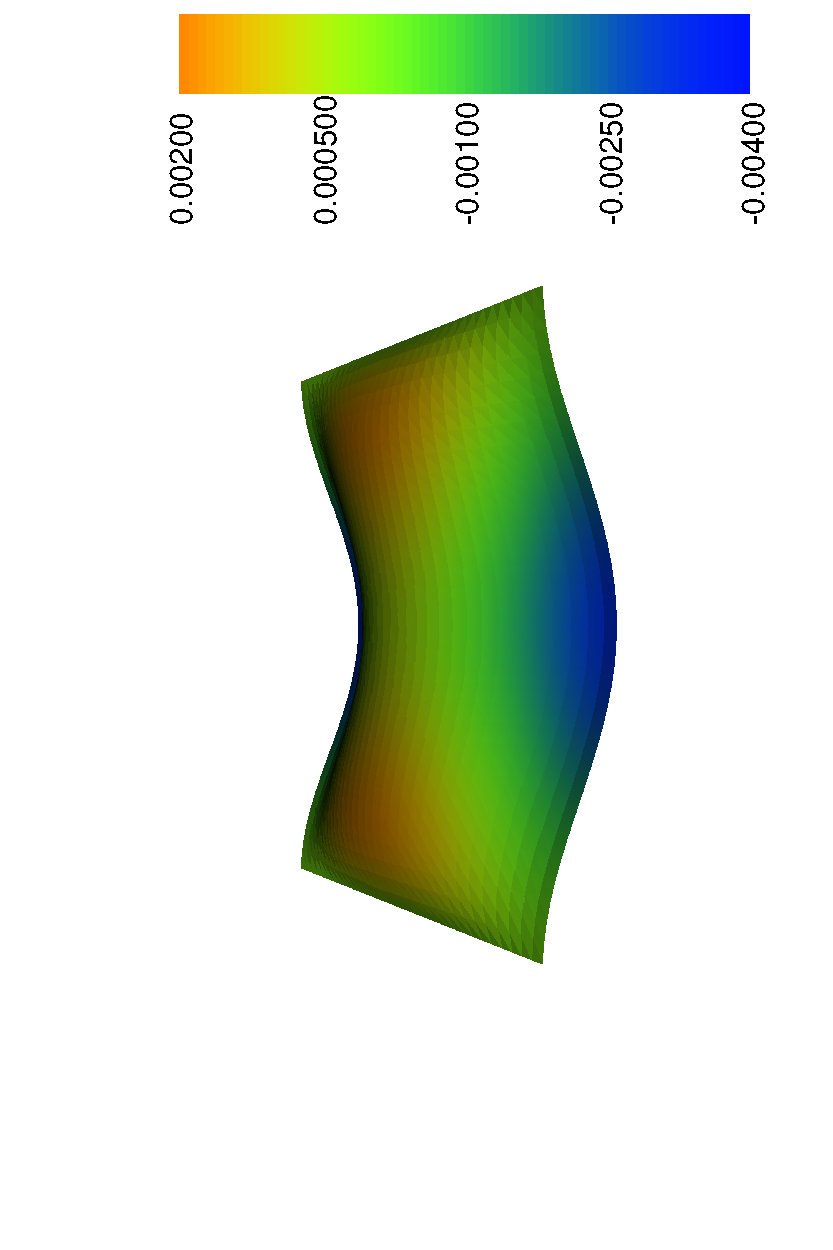
\includegraphics[scale=.6]{../FEniCS/Figures/dolfin_plot_1}
\caption{Numerical solution to (\ref{eq:poisson})}
\end{figure}


% \bibliographystyle{plain}
% \bibliography{/home/mwathen/Dropbox/MastersResearch/MHD/THESIS/ref/ref}


\chapter{Finite element discretisation}
\label{sec:discretization}

In this chapter we introduce a mixed finite element discretisation for a steady-state incompressible MHD problem that model electrically conductive fluids. Following the setting in \cite{schotzau2004mixed}, using curl-conforming elements for the magnetic field and conforming continuous elements for the velocity field. The resulting discretisation is verified though a series of numerical experiments which appear later in Chapter \ref{chap:results}. For simplicity, we only discuss in detail homogeneous Dirichlet boundary conditions, that is
\begin{equation} \label{eq:homogeneousBC}
    \uu{u} = \uu{0} \quad \mbox{and} \quad \uu{n}\times \uu{b} = \uu{0}.
\end{equation}
Inhomogeneous conditions as in \eqref{eq:bc} can be incorporated in a straightforward fashion.


\section{Variational formulation}
\label{sec:variation}

To express \eqref{eq:mhd}, \eqref{eq:bc} in weak form we follow \cite{schotzau2004mixed} and denote the $L^2$ inner product on $L^2(\Omega)^d$ by $(\cdot,\cdot)_\Omega$, for $d = 2,3$. We introduce the standard Sobolev spaces
\begin{equation} \label{eq:FuncSpace} \nonumber
 \left. \begin{aligned}
\uu{V}&=H_0^1(\Omega)^d=\left\{\,\uu{u}\in H^1(\Omega)^d\,:\,\text{$\uu{u}=\uu{0}$ on $\partial\Omega$}\,\right\},\\
Q&=L^2_0(\Omega)=\{\,p\in L^2(\Omega)\,:\,(p\,,1)_\Omega=0\,\},\\
\uu{C}&=H_0({\rm curl};\Omega) = \left\{\,\uu{b}\in L^2(\Omega)^d\,:\,\nabla\times\uu{b}\in L^2(\Omega)^{2d-3}, \
\text{$\uu{n}\times\uu{b}=\uu{0}$ on $\partial\Omega$}\,\right\},\\
S&=H^1_0(\Omega)=\{\,r\in H^1(\Omega)\,:\,r=0\ \mbox{on $\partial\Omega$}\,\},
 \end{aligned}
 \right.
 \qquad \text{}
\end{equation}
We write $\|\cdot\|_{L^2(\Omega)}$, $\|\cdot\|_{H^1(\Omega)}$ and $\|\cdot\|_{H(\rm{curl};\Omega)}$ for the associated natural norms. More precisely, for a vector fields $\uu{u},\uu{b}$ and a scalar functions $r$ the norms are defined as follows:
\begin{equation} \nonumber
 \left. \begin{aligned}
    \|\uu{u}\|_{L^2 (\Omega)} &= \left({\int_{\Omega} \uu{u}\cdot\uu{u}\;dx}\right)^{\frac{1}{2}},\\
   \|\uu{u}\|_{H^1(\Omega)} &=  \left(\|\uu{u}\|_{L^2(\Omega)}^2 + \|\nabla  \uu{u}\|_{L^2(\Omega)}^2 \right)^{\frac{1}{2}},\\
   \|\uu{b}\|_{H(\rm{curl},\Omega)} &=  \left(\|\uu{b}\|_{L^2(\Omega)}^2 + \|\nabla \times \uu{b}\|_{L^2(\Omega)}^2 \right)^{\frac{1}{2}}, \\
    \|r\|_{L^2 (\Omega)} &= \left({\int_{\Omega} r^2\;dx}\right)^{\frac{1}{2}},\\
    \|r\|_{H^1(\Omega)} &=  \left(\|r\|_{L^2(\Omega)}^2 + \|\nabla  r\|_{L^2(\Omega)}^2 \right)^{\frac{1}{2}},\\
 \end{aligned}
 \right.
 \qquad \text{}
\end{equation}
where $\|\nabla  \uu{u}\|_{L^2(\Omega)}^2$ is the $L^2$-norm of the gradient tensor $\nabla \uu{u}$. The weak formulation of the incompressible MHD system (\ref{eq:mhd}) and the boundary conditions (\ref{eq:bc}) consists in finding~$(\uu{u},p,\uu{b},r)\in \uu{V} \times Q\times \uu{C} \times S$ such that
\begin{subequations}
\label{eq:weak}
\begin{eqnarray}
\label{eq:weak1} A(\uu{u},\uu{v}) + O(\uu{u};\uu{u},\uu{v})
+C(\uu{b};\uu{v},\uu{b})
+B(\uu{v}, p) & =& (\uu{f}, \uu{v})_{\Omega},\\[.1cm]
\label{eq:weak2}
B(\uu{u},q)&=&0, \\[.1cm]
\label{eq:weak3}
M(\uu{b},\uu{c})-C(\uu{b};\uu{u},\uu{c})+D(\uu{c},r)&=& (\uu{g},\uu{c})_\Omega, \\[.1cm]
\label{eq:weak4} D(\uu{b},s)&=&0,
\end{eqnarray}
\end{subequations}
for all $(\uu{v},q,\uu{c},s)\in \uu{V} \times Q\times \uu{C}\times
S$. The individual variational forms are given by
\begin{alignat*}2\nonumber
&A(\uu{u},\uu{v})=  \int_\Omega \nu \, \nabla\uu{u}:
\nabla\uu{v}\,d\uu{x},&\qquad  & O(\uu{w};\uu{u},\uu{v}) = \int_\Omega
(\uu{w}\cdot\nabla)\uu{u} \cdot\uu{v} \, d\uu{x},
\\[.1cm]
&  B(\uu{u},q) = -\int_\Omega\,(\nabla\cdot\uu{u}) \,q \,d\uu{x},
&\qquad  &
 M(\uu{b},\uu{c})= \int_\Omega\, \kappa\nu_m
(\nabla\times\uu{b})\cdot(\nabla\times\uu{c})\,d\uu{x},\\[0.1cm]
& D(\uu{b},s) = \int_\Omega\, \uu{b} \cdot \nabla s\,
d\uu{x}, & \qquad &
C(\uu{d};\uu{v},\uu{b}) =  \int_\Omega \kappa\, (\uu{v}\times\uu{d})\cdot
(\nabla\times\uu{b})\, d\uu{x},
\end{alignat*}
where  $\nabla \uu{u}:\nabla \uu{u}$ is  defined as
$$\nabla \uu{u}:\nabla \uu{u} = \sum^d_{i,j=1}(\nabla \uu{u})_{ij}(\nabla \uu{u})_{ij}.$$ In \cite{schotzau2004mixed} it has been shown that this formulation of a the problem is discrete energy-stable and has a unique solution for small data.

\section{Mixed finite element discretisation}

Consider the domain $\Omega$ to be divided up into a regular and quasi-uniform mesh ${\mathcal T}_h=\{K\}$ consisting of triangles ($d = 2$) or tetrahedra ($d = 3$)  with mesh size $h$. Based on the function spaces defined in \eqref{eq:FuncSpace}, our finite element approximation will be sought in the finite spaces given by:
\begin{equation}
\label{eq:FiniteSpace}
\begin{split}
\uu{V}_h &=  \{\, \uu{u}\in H^1( \Omega)\, :\, \uu{u}|_K \in {\mathcal P}_{k}(K)^d, \, K \in{\mathcal T}_h \, \},\\[.1cm]
Q_h&=  \{\, p\in L^2(\Omega) \cap H^1(\Omega)\,:\, p|_K \in {\mathcal P}_{k-1}(K), \, K \in{\mathcal T}_h \,\},\\[.1cm]
\uu{C}_h &=  \{\, \uu{b}\in H_0({\rm curl}; \Omega) \,:\, \uu{b}|_K \in {\mathcal P}_{k-1}(K)^d \oplus \uu{R}_k(K), \, K \in{\mathcal T}_h \,\},\\[.1cm]
S_h&=  \{\, r\in H_0^1(\Omega) \,:\, r|_K \in {\mathcal P}_{k}(K), \, K \in {\mathcal T}_h \, \},
\end{split}
\end{equation}
for $k\geq 2$. Here we note that we are using ${\mathcal P_k}/{\mathcal P_{k-1}}$ Taylor-Hood elements for the fluid unknowns $(\uu{u},p)$ \cite{taylor1973numerical}. For the magnetic variables $(\uu{b},r)$ we use the curl-conforming \nedelec elements of the first kind \cite{nedelec1980mixed}. These choices of finite elements spaces $\uu{V}_h, \, \uu{C}_h, \, Q_h$ and $S_h$ imply that  we have conforming subspaces to our Sobolev spaces $\uu{V}, \, \uu{C}, \,Q$ and $S$, respectively. Then the finite element solution consists in finding $(\uu{u}_h,p_h,\uu{b}_h,r_h)\in \uu{V}_h\times Q_h\times \uu{C}_h\times S_h$ such that
\begin{subequations}
\label{eq:VariationForm}
\begin{eqnarray}
\label{eq:bn1} \hspace{-15mm} A(\uu{u}_h,\uu{v}) + \tilde{O}(\uu{u}_h;\uu{u}_h,\uu{v}) +C(\uu{b}_h;\uu{v},\uu{b}_h) +B(\uu{v}, p_h) & = & ( \uu{f},\uu{v}),\\[.1cm]
\label{eq:bn2}
B(\uu{u}_h,q)&=& 0, \\[.1cm]
\label{eq:bn3} M(\uu{b}_h,\uu{c})-C(\uu{b}_h;\uu{u}_h,\uu{c})+ D(\uu{c},r_h)&=& (\uu{g},\uu{c}),\\[.1cm]
\label{eq:bn4} D(\uu{b}_h,s)&=&0,
\end{eqnarray}
\end{subequations}
for all $(\uu{v},q,\uu{c},s)\in \uu{V}_h\times Q_h \times \uu{C}_h\times S_h$.

The forms $A, M, B, D$ and $C$ stay the same as on the continuous level. However, for the convection term $\tilde{O}(\cdot;\cdot,\cdot)$ we to modify the form $O(\uu{w};\uu{u},\uu{v})$ in a standard fashion to ensure the energy-stability property
\begin{equation} \label{eq:convection}
    \tilde{O}(\uu{w};\uu{u},\uu{u}) = 0, \quad \forall \uu{w},\uu{u} \in  \uu{V}_h.
\end{equation}
To ensure this property we integrate by parts the convection form $O(\uu{w};\uu{u},\uu{u})$  to obtain
\begin{equation} \nonumber
 \left. \begin{aligned}
     \int_\Omega (\uu{w}\cdot\nabla)\uu{u} \cdot\uu{u} \, d\uu{x} =& -\frac{1}{2}\int_{\Omega} \nabla \cdot \uu{w} \uu{u} \cdot \uu{u} \, d\uu{x}
     +\frac{1}{2}\int_{\partial \Omega} \uu{w}\cdot \uu{n} |\uu{u}|^2\, ds,
 \end{aligned}
 \right.
 \qquad \text{}
\end{equation}
recalling that $\uu{n}$ is the unit outward normal on $\partial \Omega$. Therefore, we choose the modified convection form $\tilde{O}(\uu{w};\uu{u},\uu{v})$ as
$$\tilde{O}(\uu{w};\uu{u},\uu{v}) =  \int_\Omega (\uu{w}\cdot\nabla)\uu{u} \cdot\uu{v} \, d\uu{x} +\frac{1}{2}\int_{\Omega} \nabla \cdot \uu{w} \uu{u} \cdot \uu{v}\, d\uu{x}-\frac{1}{2}\int_{\partial \Omega} \uu{w}\cdot \uu{n} \uu{u} \cdot \uu{v}\, ds.$$
By construction, the property \eqref{eq:convection} is now satisfied. Note also that for homogeneous boundary conditions as assumed in \eqref{eq:homogeneousBC}, the boundary integral term in $\tilde{O}$ can be omitted.

Again in \cite{schotzau2004mixed} it has been shown that this formulation of a MHD is discrete energy-stable and has a unique solution for small data. Also, optimal order error estimates in the mesh size $h$ have been derived for small data using the stability property \eqref{eq:convection}. Namely, for sufficiently smooth solutions, we have that
$$\|\uu{u}-\uu{u}_h\|_{H^1(\Omega)}+\|\uu{b}-\uu{b}_h\|_{H(\rm{curl};\Omega)}+\|p-p_h\|_{L^2(\Omega)}+\|r-r_h\|_{H^1(\Omega)} \leq C h^k,$$
for a constant $C>0$ independent of the mesh size. However, the $L^2$-norm error for the velocity field is of order $\mathcal{O}(h^{k+1})$ (as $\uu{V}_h$ consists of a full polynomial space on each element). In contrast, we cannot expect $L^2$-norm errors of  order $\mathcal{O}(h^{k+1})$ for the magnetic field (as $\uu{C}_h$ does not consists of a full polynomial space on each element).


\subsection{Matrix representation}

This variational formulation \eqref{eq:VariationForm} now can be converted into a matrix representation. To do this, we introduce the basis function for the finite elements spaces in \eqref{eq:FiniteSpace}:
\begin{alignat}2
\label{eq:bases1}
\uu{V}_h & = \mbox{span}\langle  \uu{\psi}_j \rangle _{j=1}^{n_u}, & \qquad &
Q_h  = \mbox{span} \langle  \alpha_i \rangle _{i=1}^{m_u},\\[0.1cm]
 \uu{C}_h& =\mbox{span}\langle \uu{\phi}_j \rangle _{j=1}^{n_b}, & \qquad & S_h = \mbox{span} \langle \beta_i
\rangle_{i=1}^{m_b}.
\end{alignat}
The aim now is to find the coefficient vectors $u = (u_1, \ldots , u_{n_u}) \in \mathbb{R}^{n_u}$, $p = (p_1, \ldots , p_{m_u}) \in \mathbb{R}^{m_u}$, $b = (b_1, \ldots , b_{n_b}) \in \mathbb{R}^{n_b}$, and $r = (r_1, \ldots , r_{m_b}) \in \mathbb{R}^{m_b}$ of the finite element functions $(\uu{u}_h, p_h,\uu{b}_h, r_h)$. As usual, this is done by writing the bilinear forms in \eqref{eq:VariationForm} in terms of the following stiffness matrices and load vectors:
\begin{alignat*}2
A_{i,j} &= A(\uu{\psi}_j,\uu{\psi}_i), &\quad  &1 \leq i,j \leq n_u,\\[0.1cm]
B_{i,j} &= B(\uu{\psi}_j,\alpha_i), &\quad &1 \leq i \leq m_u, \ 1 \leq j \leq n_u,\\[.1cm]
D_{i,j} &= D(\uu{\phi}_j,\beta_i),  & & 1 \leq i \leq m_b,\ 1 \leq j \leq n_b,\\[.1cm]
M_{i,j}&= M(\uu{\phi}_j,\uu{\phi}_i), &\qquad & 1 \leq i,j \leq n_b,\\[.1cm]
f_i &= (\uu{f},\uu{\psi}_i)_\Omega, & & 1\leq i\leq n_u,\\[.1cm]
g_i &= (\uu{g},\uu{\phi}_i)_\Omega, & & 1\leq i \leq n_b.
\end{alignat*}
For the two non-linear forms, $\tilde{O}$ and $C$, we define the corresponding stiffness matrices with respect to given finite element functions $\uu{w} \in \uu{V}_h$ and $\uu{d}_h\in \uu{C}_h$ in the first argument and their associated coefficient vectors $w$ and $d$ as
\begin{alignat*}2
O(w)_{i,j} &=\tilde{O}(\uu{w};\uu{\psi}_j,\uu{\psi}_i), &\quad  &1 \leq i,j \leq n_u,\\[.1cm]
C(d)_{i,j} &= C(\uu{d};\uu{\psi}_j,\uu{\phi}_i), & & 1\leq i \leq n_b,\ 1 \leq j \leq n_u.
\end{alignat*}

Thus, the numerical solution to \eqref{eq:mhd} consists in solving the non-linear system
\begin{equation}
\label{eq:matrix-system}
\left(
\begin{array}{cccc}
A+O(u) & B^T & C^T(b) & 0\\
B & 0 & 0 & 0\\
-C(b) & 0 & M & D^T \\
0 & 0 & D & 0
\end{array}
\right)
\,
\left(
\begin{array}{c}
u\\
p\\
b\\
r
\end{array}
\right) =
\left(
\begin{array}{c} f\\0\\g\\0
\end{array}
\right).
\end{equation}
where the vectors  $u\in\mathbb{R}^{n_u}$, $p\in\mathbb{R}^{m_u}$,  $b\in\mathbb{R}^{n_b}$, and $r\in\mathbb{R}^{m_b}$ are the unknown coefficients of the finite element functions. We shall omit the dependence of $O$ and $C$ on $b$ and $u$, respectively, and simply  write $O$ and $C$.

\section{Picard iteration (P)}
\label{sec:nonlinear}
The discrete system \eqref{eq:matrix-system} is non-linear, and therefore appling a non-linear solver to this problem is necessary. A common choice to deal with the non-linearity within the incompressible Navier-Stokes equations in isolation is to perform Oseen or Picard iterations \cite{elman2005finite}. This involves linearising around the current velocity and solving for updates.

We adapt this approach for the full MHD system as well. Given a current iterate $(\uu{u}_h,p_h,\uu{b}_h,r_h)$  we solve for updates $(\delta \uu{u}_h,\delta p_h,\delta \uu{b}_h,\delta r_h)$ and introduce the next iterate by setting:
\begin{equation}\nonumber
\begin{array}{cc}
% \label{eq:updates}
\uu{u}_h& \hspace{-3mm} \rightarrow \uu{u}_h +\delta \uu{u}_h, \quad p_h \rightarrow p_h +\delta p_h,\\
\uu{b}_h& \hspace{-3mm}  \rightarrow \uu{b}_h +\delta \uu{b}_h, \quad r_h \rightarrow r_h +\delta r_h.
\end{array}
\end{equation}
In variational form, the updates $(\delta \uu{u}_h,\delta p_h,\delta \uu{b}_h,\delta r_h)\in \uu{V}_h\times Q_h \times \uu{C}_h\times S_h$ are found by solving the Picard system (P):
\begin{equation} \nonumber
% \label{eq:picard}
\begin{split}
A(\delta\uu{u}_h, \uu{v}) +\tilde{O}(\uu{u};\delta\uu{u}_h,\uu{v})+ C(\uu{b}_h;\uu{v},\delta \uu{u}_h) + B(\uu{v}, \delta p_h) & = R_u(\uu{u}_h,\uu{b}_h,p_h;\uu{v}),\\[.1cm]
B(\delta\uu{u}_h,q)&= R_p(\uu{u}_h;q), \\[.1cm]
M(\delta \uu{b}_h,\uu{c})+
D(\uu{c},\delta r_h)-C(\uu{b}_h;\delta \uu{u}_h,\uu{v})&= R_b(\uu{u}_h,\uu{b}_h,r_h;\uu{c}),\\[.1cm]
D(\delta \uu{b}_h,s)&= R_r(\uu{b}_h;s),
\end{split}
\end{equation}
for all $(\uu{v},q,\uu{c},s)\in \uu{V}_h\times Q_h \times \uu{C}_h\times S_h$. The right hand side linear forms correspond to the residual at the current iteration $(\uu{u}_h,p_h,\uu{b}_h,r_h)$ defined by:
\begin{align*}
 R_u(\uu{u}_h,\uu{b}_h,p_h;\uu{v})&=(\uu{f}, \uu{v})_\Omega-A(\uu{u}_h,\uu{v})
-  \tilde{O}(\uu{u}_h;\uu{u}_h,\uu{v})  - C(\uu{b}_h;\uu{v},\uu{b}_h)-B(\uu{v},p_h),\\[.1cm]
R_p(\uu{u}_h;q)&=-B(\uu{u}_h,q),\\[.1cm]
 R_b(\uu{u}_h,\uu{b}_h,r_h;\uu{c})&=(\uu{g,c})_\Omega -M(\uu{b}_h,\uu{c})
+ C(\uu{b}_h;\uu{u}_h,\uu{c})-D(\uu{c},r_h),\\[.1cm]
R_r(\uu{b}_h;s)&=-D(\uu{b}_h,s),
\end{align*}
for all $(\uu{v},q,\uu{c},s)\in \uu{V}_h\times Q_h \times \uu{C}_h\times S_h$.

In \cite{schotzau2004mixed} it is shown that for small data the Picard iteration (P) will converge to the exact solution given any initial guess.

To formulate the variational form of the Picard iteration (P) in matrix form, let $({u},p,{b},r)$ be the coefficient vectors associated with $(\uu{u}_h,p_h,\uu{b}_h,r_h)$ and $(\delta{u},\delta p,\delta{b},\delta r)$ be the coefficient vectors of $(\delta \uu{u}_h,\delta p_h,\delta \uu{b}_h,\delta r_h)$, then it can readily seen that the Picard iteration (P) amounts to solving the matrix system
\begin{equation}
\label{eq:mhd_saddle}
%\mathcal{K} x \equiv
\left(
\begin{array}{cccc}
A+O & B^T & C^T & 0\\
B & 0 & 0 & 0 \\
-C & 0 & M & D^T\\
0 & 0 & D & 0
\end{array}
\right)
\,
\left(
\begin{array}{c}
\delta u\\
\delta p\\
\delta b\\
\delta r
\end{array}
\right)  =
\begin{pmatrix}
r_u \\
r_p\\
r_b\\
r_r
\end{pmatrix},
\end{equation}
with
\begin{align*}
r_u &= f- Au -O(u) u - C(b)^T b- B^T p,\\[0.1cm]
r_p &=-B u,\\[0.1cm]
r_b &=g-Mu+C(b)b-D^T r,\\[0.1cm]
r_r &=-D b.
\end{align*}
Here, the matrix $A$  is symmetric positive-definite (SPD), $O$ is non-symmetric and $-C,C^T$ appear in a skew symmetric fashion. We also note that $M$ is symmetric positive-semidefinite (SPSD) with nullity $m_b$ corresponding to the discrete gradients.


\section{Decoupled iterations}
\label{sec:FEMdecouple}


The full MHD system \eqref{eq:mhd}, \eqref{eq:bc} is a coupled system consisting of the incompressible Navier-Stokes and Maxwell's equations, coupled through the non-linear skew symmetric coupling term $C$. In addition, the convection term $O$ is non-linear as well. These two terms make the numerical solution challenging. Therefore, if one or both of these terms is small then it may be possible to iterate explicitly. In particular if the coupling term, $C$, is small then we may completely decouple the system into a Navier-Stokes problem and a Maxwell problem. The two resulting decoupling schemes are what we call Magnetic and Complete Decoupling and are both described below.


\subsection{Magnetic decoupling (MD)}
\label{sec:FEMmd}

Consider the first situation where there is  weak coupling within the system, that is when $C$ is small. Then it may be possible to drop these terms to completely decouple the system into the two subproblems, the Navier-Stokes and Maxwell's equations. We will call this Magnetic decoupling.
% For a given solution $(\uu{u}_h,p_h,\uu{b}_h,r_h)$, neglecting the coupling terms in \eqref{eq:picard} results in solving for the updates $(\delta \uu{u}_h,\delta p_h,\delta \uu{b}_h,\delta r_h) \in \uu{V}_h \times Q_h \times \uu{C}_h \times S_h$  such that
% \begin{equation}
% \label{eq:picard_explicit_MD}
% \begin{split}
% A(\delta\uu{u}_h, \uu{v}) +O(\uu{u};\delta\uu{u}_h,\uu{v})+ B(\uu{v}, \delta p_h) & = R_u(\uu{u}_h,\uu{b}_h,p_h;\uu{v})\\[.1cm]
% B(\delta\uu{u}_h,q)&= R_p(\uu{u}_h;q), \\[.1cm]
% M(\delta \uu{b}_h,\uu{c})+
% D(\uu{c},\delta r_h)&= R_b(\uu{u}_h,\uu{b}_h,r_h;\uu{c}),\\[.1cm]
% D(\delta \uu{b}_h,s)&=R_r(\uu{b}_h;s),
% \end{split}
% \end{equation}
% where again $(\uu{v},q,\uu{c},s)\in\uu{V}_h\times Q_h\times\uu{C}_h\times S_h$ and $R_u$, $R_p$, $R_b$ and $R_r$ which are defined in section \ref{sec:nonlinear}. Again, let $({u},p,{b},r)$ be the coefficient vectors of $(\uu{u}_h,p_h,\uu{b}_h,r_h)$ and $(\delta{u},\delta p,\delta{b},\delta r)$ be the coefficient vectors of $(\delta \uu{u}_h,\delta p_h,\delta \uu{b}_h,\delta r_h)$, then this amounts to solving the linear system:
Then \eqref{eq:mhd_saddle} amounts
\begin{equation}
\label{eq:matrix_MD}
%\mathcal{K} x \equiv
\left(
\begin{array}{cccc}
A+O(u) & B^T & 0 & 0\\
B & 0 & 0 & 0 \\
0 & 0 & M & D^T\\
0 & 0 & D & 0
\end{array}
\right)
\,
\left(
\begin{array}{c}
\delta u\\
\delta p\\
\delta b\\
\delta r
\end{array}
\right)  =
\begin{pmatrix}
r_u \\
r_p\\
r_b\\
r_r
\end{pmatrix},
\end{equation}
with
\begin{align*}
r_u &= f- Au -O u - C^T b- B^T p,\\[0.1cm]
r_p &=-B u,\\[0.1cm]
r_b &=g-Mu+Cb-D^T r,\\[0.1cm]
r_r &=-D b.
\end{align*}
From \eqref{eq:matrix_MD} we can see that the system is now completely decoupled. This enable us to apply solve each individual subproblem separately and possibly in parallel.

\subsection{Complete decoupling}


For the second decoupling scheme, we again consider there to be weak coupling of the system but we also consider that the fluid equations are diffusion dominated and hence can exclude the convection terms.
% This is the simplest technique as it removes all non-linear terms. Again, for a given solution $(\uu{u}_h,p_h,\uu{b}_h,r_h)$, removing the coupling and convection terms in \eqref{eq:picard} results in solving for the updates $(\delta \uu{u}_h,\delta p_h,\delta \uu{b}_h,\delta r_h) \in \uu{V}_h \times Q_h \times \uu{C}_h \times S_h$  such that
% \begin{equation}
% \label{eq:picard_explicit_CD}
% \begin{split}
% A_h(\delta\uu{u}_h, \uu{v}) + B(\uu{v}, \delta p_h) & = R_u(\uu{u}_h,\uu{b}_h.p_h;\uu{v})\\[.1cm]
% B(\delta\uu{u}_h,q)&= R_p(\uu{u}_h;q), \\[.1cm]
% M(\delta \uu{b}_h,\uu{c})+
% D(\uu{c},\delta r_h)&= R_b(\uu{u}_h,\uu{b}_h,r_h;\uu{c}),\\[.1cm]
% D(\delta \uu{b}_h,s)&=R_r(\uu{b}_h;s),
% \end{split}
% \end{equation}
% where $(\uu{v},q,\uu{c},s)\in\uu{V}_h\times Q_h\times\uu{C}_h\times S_h$.  Taking $({u},p,{b},r)$ as the coefficient vectors of $(\uu{u}_h,p_h,\uu{b}_h,r_h)$ and $(\delta{u},\delta p,\delta{b},\delta r)$ be the coefficient vectors of $(\delta \uu{u}_h,\delta p_h,\delta \uu{b}_h,\delta r_h)$, then the proposed decoupled linear system is
This amounts to
\begin{equation}
\label{eq:matrix_CD}
%\mathcal{K} x \equiv
\left(
\begin{array}{cccc}
A & B^T & 0 & 0\\
B & 0 & 0 & 0 \\
0 & 0 & M & D^T\\
0 & 0 & D & 0
\end{array}
\right)
\,
\left(
\begin{array}{c}
\delta u\\
\delta p\\
\delta b\\
\delta r
\end{array}
\right)  =
\begin{pmatrix}
r_u \\
r_p\\
r_b\\
r_r
\end{pmatrix},
\end{equation}
with
\begin{align*}
r_u &= f- Au -O u - C^T b- B^T p,\\[0.1cm]
r_p &=-B u,\\[0.1cm]
r_b &=g-Mu+Cb-D^T r,\\[0.1cm]
r_r &=-D b.
\end{align*}
This is the simplest technique as it removes all non-linear terms and hence leaves the linear Stokes problem in the upper $(1,1)$ block matrix.

In this chapter we have introduced a mixed finite element approximation to the full MHD system given in \eqref{eq:mhd} and \eqref{eq:bc}. We followed the mixed approach outlined in \cite{schotzau2004mixed} and expressed the MHD system in the matrix form \eqref{eq:mhd_saddle}. Using the Picard iteration  \eqref{eq:mhd_saddle} we introduced two possible decoupling schemes which maybe simpler to solve for depending on the parameters ($\kappa$, $\nu$ and $\nu_m$). The next chapter will discuss possible preconditioning approaches to these systems.
 \chapter{Linear Solver}

In many applications one of the main problems is to find the solution of a linear system. This system may arise form an optimisation or, like here, a discretised PDE. In this chapter we will go through the two methods which this is done.

\section{Direct Methods}

Suppose you are given a linear system of the form
$$Ax = b$$
where $A$ is a real $n\times n$ non-singular matrix and right hand side vector $b \in \mathcal{R}^n$, where the aim is to solve for the vector $x \in \mathcal{R}^n$. All direct methods are based on Gaussian elimination.

\subsection{Software}

UMFPACK \cite{Davis:2004:CPS:992200.992205,Davis:2004:AUV:992200.992206,Davis:1999:CUM:305658.287640,davis1997unsymmetric}, PASTIX \cite{henon2002pastix}, SuperLU \cite{superlu_ug99,li05} and MUMPS \cite{amestoy2000multifrontal,amestoy2001fully,amestoy2006hybrid}


\section{Iterative Methods}





\chapter{Preconditioning}
\label{chap:precond}

% Let us define the matrix of the linear system \eqref{eq:mhd_saddle} as $\mathcal{K}$.




The linear system \eqref{eq:mhd_saddle} is typically sparse and of large dimension, hence to efficiently solve for it we use a preconditioned iterative approach as proposed in \cite{li2010numerical}. We start by reviewing some preconditioning strategies for the incompressible Navier-Stokes and Maxwell subproblems in isolation. From these techniques we will then introduce and  numerically test  preconditioners for the full MHD system.

\section{Navier-Stokes equations}
\label{sec:NSprecond}


To start with, consider the steady state incompressible Navier-Stokes equations in isolation. Let
\begin{equation}
\label{eq:ns_coeff}
\mathcal{K}_{\rm NS}=
\begin{pmatrix}
F & B^T \\
B & 0
\end{pmatrix},
\end{equation}
be the discretised and linearised Navier-Stokes subproblem where $F~=~A~+~O$. Due to the convection term, $O$, this  system is non-symmetric and we will use GMRES to solve this subproblem \cite{saad1986gmres}. An excellent choice for a preconditioner for a saddle point system like this is to use a block diagonal or block triangular based preconditioner of the form
\begin{equation}
\label{eq:ns_pc_upper}
\mathcal{M}_{\rm NS} =
\begin{pmatrix}
F & B^T \\
0 & -S
\end{pmatrix},
\end{equation}
where the Schur complement $S$ is given by $S=B F^{-1} B^T$. It has been proved in \cite{murphy2000note} that for a suitable Krylov subspace method then the iterative scheme will converge in exactly $2$ iterations when using the block triangular preconditioner or $3$ iterations using a block diagonal where the $B^T$ is dropped from the $(1,2)$ block in $\mathcal{M}_{\rm NS}$.

In practice it is often too expensive to form and solve for the Schur complement, hence, a good approximation to it is needed. Two well known preconditioners for the incompressible Navier-Stokes equations are the Least Squares Commutator (LSC) and the Pressure Convection-Diffusion (PCD) preconditioners. Both can be found in \cite{elman2005finite} and we will just outline the procedure how these can be applied on the discrete level.

% Both methods (LSC and PCD)  start with the convection-diffusion operator associated with the velocity space $\uu{V}_h$ given by
% $$\mathcal{L} = -\nu \Delta +\uu{w} \cdot \nabla\, .$$
% As before $\uu{w}$ is the discrete velocity calculated at the previous non-linear iteration. Suppose that there is a corresponding operator defined in the pressure space
% $$\mathcal{L}_p = (-\nu \Delta +\uu{w} \cdot \nabla)_p\, .$$
% Consider the commutator of the convection-diffusion operator associated with the gradient operator
% \begin{equation} \label{eq:ContCommutator}
% \epsilon = (-\nu \Delta +\uu{w} \cdot \nabla)\nabla - \nabla (-\nu \Delta +\uu{w} \cdot \nabla)_p
% \end{equation}
% to be small. In fact, if $\uu{w}$ was constant then $\epsilon = 0$. We will be using \eqref{eq:ContCommutator} to derive both LSC and PCD.



\subsection{Pressure Convection-Diffusion (PCD)}
Before considering the PCD approach to approximate the Schur complement, we define the velocity mass matrix as $Q=(Q_{i,j})_{i,j=1}^{n_u} \in{\mathbb R}^{n_u \times n_u}$, where in terms of the basis $\{\uu{\psi_i}\}$
\begin{equation}
\label{eq:pressure_mass}
Q_{i,j}=
\int_\Omega\, \uu{\psi_j}\cdot \uu{\psi_i} \,d\uu{x}, \quad 1\leq i,j \leq n_u.
\end{equation}
In \cite[Chap. 8]{elman2005finite} the discrete commutator of the convection-diffusion operator associated with the gradient operation is introduced and given by
\begin{equation} \label{eq:DisCommutator}
    \epsilon_h = (Q^{-1}F)(Q^{-1}B^T)-(Q^{-1}B^T)(W^{-1}F_p)
\end{equation}
In this equation, $W=(W_{i,j})_{i,j=1}^{m_u} \in{\mathbb R}^{m_u \times m_u}$, $F_p=((F_{p})_{i,j})_{i,j=1}^{m_u} \in{\mathbb R}^{m_u \times m_u}$ and introduce $A_p=((A_{p})_{i,j})_{i,j=1}^{m_u} \in{\mathbb R}^{m_u \times m_u}$ (which will be used later) are mass matrix, convection diffusion operator and Laplacian matrix defined on the pressure space as:
\begin{equation}
\label{eq:PressureMass}
 \left. \begin{aligned}
W_{i,j}&= \int_\Omega\, \alpha_j \alpha_i \,dx, \ \ 1\leq i,j \leq m_u, \\
(F_{p})_{i,j}&= \nu \int_\Omega\, \grad \alpha_j \cdot \grad \alpha_i +(\uu{w} \cdot \grad \alpha_j)\alpha_i\,dx,\ \ 1\leq i,j \leq m_u, \\
(A_{p})_{i,j}&=  \int_\Omega\, \grad \alpha_j \cdot \grad \alpha_i \,dx, \ \ 1\leq i,j \leq m_u.
 \end{aligned}
 \right.
 \qquad \text{}
\end{equation}
These matricies are well-defined since our pressure spaces are continuous. Assuming that the commutator is small then pre and post multiplying \eqref{eq:DisCommutator} by $B F^{-1} Q$ and $F_p^{-1}W$, respectively, lets us separate the Schur complement to give
\begin{equation} \label{eq:SchurApprox}
    BF^{-1}B^T \approx B Q^{-1}B^T F_p^{-1} W.
\end{equation}

In general, $BF^{-1}B$ is both costly to form and usually dense, so it is impractical to use.  Our discretisation is inf-sup stable which means that there is spectral equivalency between $BQ^{-1}B^T$ and the pressure Laplacian, $A_p$, see \cite[Section 5.5.1]{elman2005finite}. Hence, the Schur complement can be approximated by:
$$S_{\rm PCD} =A_p F_p^{-1}W.$$
Applying the PCD preconditioner to the full Navier-Stokes system involves solving the system
\begin{equation} \nonumber
% \label{eq:matrix-system}
\left(
\begin{array}{cc}
F & B^T \\
0 & -A_p F_p^{-1}W
\end{array}
\right)
\,
\left(
\begin{array}{c}
x \\
y
\end{array}
\right) =
\left(
\begin{array}{c}a\\b
\end{array}
\right)
\end{equation}
at each Krylov iteration. This can be solved  efficiently by splitting it into the following two steps
\begin{itemize} \label{it:PCDsolve}
    \item[1.] Solve for $y$: $y = -W^{-1}F_p A_p^{-1}b$
    \item[2.] Solve for $x$: $x = F^{-1}(a-B^Ty).$
\end{itemize}
This means that we have one pressure Poisson solve ($A_p^{-1}$), one mass matrix solve ($W^{-1}$) and one convection-diffusion solve ($F^{-1}$) at each Krylov iteration. These solves will be done using direct solver unless specifically stated otherwise.

\subsection{Least Squares Commutator}

As for the derivation of the PCD preconditioner we start off with the discrete commutator of the convection-diffusion operator
\begin{equation} \nonumber
    \epsilon_h = (Q^{-1}F)(Q^{-1}B^T)-(Q^{-1}B^T)(W^{-1}F_p).
\end{equation}
Suppose that the $Q$-norm is defined by $\|v\|_{Q} = (Qv,v)^{\nicefrac{1}{2}}$. Then this time we minimise $\epsilon_h$ in the $Q$-norm to try to find an expression for $F_p$. The minimisation is given by
$$\min \|(Q^{-1}F)(Q^{-1}B^T)-(Q^{-1}B^T)(W^{-1}F_p) \|_Q.$$
Solving this optimisation problem, as shown in \cite{elman2005finite}, is equivalent to solving the following normal equations
$$W^{-1}BQ^{-1}B^TW^{-1}F_p = W^{-1}BQ^{-1} FQ^{-1}B^T.$$
This yields the following expression for $F_p$:
$$F_p = W(BQ^{-1}B^T)^{-1}(BQ^{-1} FQ^{-1}B^T).$$
By substitution this into expression \eqref{eq:SchurApprox} we obtain the LSC approximation to the Schur complement:
\begin{equation} \nonumber
    S = BF^{-1}B^T \approx S_{\rm LSC} = (B Q^{-1} B^T)(BQ^{-1}FQ^{-1}B^T)^{-1}(B Q^{-1} B^T).
\end{equation}
Therefore, applying the LSC preconditioner to the full Navier-Stokes system $\mathcal{K}_{\rm NS}$ in \eqref{eq:ns_coeff} involves solving for the matrix
\begin{equation} \nonumber
\left(
\begin{array}{cc}
F & B^T \\
0 & -S_{\rm LSC}
\end{array}
\right)
\,
\left(
\begin{array}{c}
x \\
y
\end{array}
\right) =
\left(
\begin{array}{c}a\\b
\end{array}
\right)
\end{equation}
at each Krylov iteration. Again, this can be split up into the following two steps:
\begin{itemize}
    \item[1.] Solve for $y$: $y = -(B Q^{-1} B^T)^{-1}(BQ^{-1}FQ^{-1}B^T)(B Q^{-1} B^T)^{-1}b$
    \item[2.] Solve for $x$: $x = F^{-1}(a-B^Ty).$
\end{itemize}
Hence, we have two pressure Poisson solves ($(B Q^{-1} B^T)^{-1}$) and one Convection-Diffusion solve ($F^{-1}$) at each Krylov iteration. In practice, we take the diagonal or lumped diagonal of $Q$ to form $B Q^{-1} B^T$. These solves, as in with the PCD preconditioner, will be done directly.


\section{Maxwell's equations}
\label{sec:MaxwellPrecond}

Next, consider the Maxwell subproblem
\begin{equation}
\label{eq:m_coeff}
\mathcal{K}_{\rm MX}=
\begin{pmatrix}
M & D^T \\
D & 0
\end{pmatrix}.
\end{equation}
As for the Navier-Stokes subproblem in Section \ref{sec:NSprecond}, we apply a block preconditioning strategy for $\mathcal{K}_{\rm MX}$ in  \eqref{eq:m_coeff}.

Recall that the $(1,1)$ block of $\mathcal{K}_{\rm MX}$ is the curl-curl operator, and hence the matrix $M$ is singular with nullity $m_b$ which corresponds to the discrete gradients. Therefore the usual Schur complement does not exist as it involves inverting $M$. To overcome this difficulty, we employ the approach in  \cite{golub2003solving,greif2006preconditioners} based on  augmentation. More precisely, we replace $M$ by $M+D^T\mathcal{W}^{-1}D$ where $\mathcal{W}\in {\mathbb R}^{m_b\times m_b}$ is a symmetric positive definite matrix, see \cite{golub2003solving,greif2006preconditioners} for more details. The addition of the matrix ($D^T\mathcal{W}^{-1}D$) removes the singularity of the $(1,1)$ block of $\mathcal{K}_{\rm MX}$ without changing the solution (since $Db = 0$). For the Maxwell subproblem the appropriate choice of $\mathcal{W}$ is the scalar Laplacian on $S_h$ defined as $L=(L_{i,j})_{i,j=1}^{m_b} \in{\mathbb R}^{m_b \times m_b}$ with
\begin{equation}
\label{eq:scalar_laplace}
L_{i,j}=\int_\Omega\,\nabla\beta_j\cdot\nabla\beta_i\,d\uu{x},
\end{equation}
see  \cite{greif2007preconditioners}. Therefore we will consider preconditioning the following augmented system:
\begin{equation}
\label{eq:AugmentMaxwell}
\bar{\mathcal{K}}_{\rm MX}=
\begin{pmatrix}
M + D^TL^{-1}D & D^T \\
D & 0
\end{pmatrix}.
\end{equation}

\subsection{An ideal preconditioner}


It has been shown in \cite{greif2007preconditioners} that an ideal preconditioner for $\bar{\mathcal{K}}_{\rm MX}$ in \eqref{eq:AugmentMaxwell} is the block diagonal matrix
\begin{equation}
\label{eq:maxwell_pc_ideal}
\mathcal{M}_{\rm iMX} =
\begin{pmatrix}
M+D^T L^{-1} D & 0 \\
0 & L
\end{pmatrix}.
\end{equation}
Applying \eqref{eq:maxwell_pc_ideal} as the preconditioner yields exactly two eigenvalues, $1$ and $-1$. Therefore using this matrix as a preconditioner means that MINRES will converge in two iterations  \cite{paige1975solution}. However, forming the matrix $M+D^T L^{-1} D$ is costly, hence, $\mathcal{M}_{\rm iMX}$  is  impractical  for large systems.


\subsection{A practical preconditioner}

A good approximation for $M+D^T L^{-1} D$ is required to make the ideal preconditioner, $\mathcal{M}_{\rm iMX}$, suitable in practise. It has been shown in \cite{greif2007preconditioners}  that $M+D^T L^{-1} D$ is spectrally equivalent to $M+X$  where $X=(X_{i,j})_{i,j=1}^{n_b}\in{\mathbb R}^{n_b \times n_b}$ is the mass matrix on the magnetic space and is defined as
\begin{equation}
\label{eq:magnetic_mass}
X_{i,j}=\int_\Omega\, \uu{\psi}_j\cdot\uu{\psi}_i\,d\uu{x}.
\end{equation}
Using this approximation leads to the practical preconditioner
\begin{equation}
\label{eq:maxwell_pc_X}
\mathcal{M}_{\rm MX} =
\begin{pmatrix}
N& 0 \\
0 & L
\end{pmatrix},
\end{equation}
where $N = M+X$.

\section{A preconditioner for the MHD problem}
\label{sec:MHDprecond}

Sections \ref{sec:NSprecond} and \ref{sec:MaxwellPrecond} looked briefly at the preconditioning strategies for the Navier-Stokes and Maxwell's equations. Using these techniques we will look at possible scalable preconditioners for the full MHD problem,
\begin{equation}
    {\mathcal K}_{\rm MH} = \left(
\begin{array}{cccc}
A+O & B^T & C^T & 0\\
B & 0 & 0 & 0\\
-C & 0 & M & D^T \\
0 & 0 & D & 0
\end{array}
\right).
\end{equation}
Using the Navier-Stokes and Maxwell subproblem preconditioners \eqref{eq:ns_pc_upper} and \eqref{eq:maxwell_pc_X} respectively, then we propose the following preconditioner for ${\mathcal K}_{\rm MH}$
\begin{equation}
\label{eq:mhd_pc_ls}
\mathcal{M}_{\rm MH} =
\left(
\begin{array}{cccc}
F & B^T & C^T & 0\\
0 & -S & 0 & 0 \\
-C & 0 & N & 0\\
0 & 0 & 0 & L
\end{array}
\right).
\end{equation}
Due to the coupling terms, $C$, the application of this precondioner is hard. To overcome this, we propose to invert  $\mathcal{M}_{\rm MH}$ by means of an inner preconditioner Krylov solver. The inner preconditioner is given by
\begin{equation}
\label{eq:mhd_pc_inner}
\mathcal{M}_{\rm innerMH} =
\left(
\begin{array}{cccc}
F & B^T & 0 & 0\\
0 & -{S} & 0 & 0 \\
0 & 0 & N & 0\\
0 & 0 & 0 & L
\end{array}
\right).
\end{equation}

\section{Preconditioners for MD and CD}

In Section \ref{sec:FEMdecouple} we introduced two decoupling schemes, namely Magnetic Decoupling (MD) and Complete Decoupling (CD). Using the results from sections \ref{sec:MaxwellPrecond} and \ref{sec:NSprecond} we will discuss the preconditioning approaches that we imply for these decoupling schemes.

\subsection{Magnetic decoupling}
\label{sec:MDprecond}

From section \ref{sec:FEMmd} the the matrix to be preconditioned is as follows:
\begin{equation}
   \mathcal{K}_{\rm MD} =
    \left(
    \begin{array}{cccc}
    F& B^T & 0 & 0\\
    B & 0 & 0 & 0 \\
    0 & 0 & M & D^T\\
    0 & 0 & D & 0
    \end{array}
    \right).
\end{equation}
Recall that removing the coupling terms completely decouples the system. This therefore enables us to use the optimal preconditioners for each of the subproblems separately and in parallel. Using the subproblem preconditioners \eqref{eq:maxwell_pc_X} and \eqref{eq:ns_pc_upper} then the optimal preconditioner for $\mathcal{K}_{\rm MD}$ is
\begin{equation}
\label{eq:mhd_pc_explicit}
\mathcal{M}_{\rm MD} =
\left(
\begin{array}{cccc}
F & B^T & 0 & 0\\
0 & -{S} & 0 & 0 \\
0 & 0 & N & 0\\
0 & 0 & 0 & L
\end{array}
\right).
\end{equation}


\subsection{Complete decoupling}
\label{sec:CDprecond}

To form an appropriate preconditioner for the CD iteration in \eqref{eq:matrix_CD} we first need to consider how to deal with the upper $(2,2)$ block matrix which corresponds to the discrete Stokes equations
\begin{equation}\nonumber
   \mathcal{K}_{\rm S} =
    \left(
    \begin{array}{cc}
    A& B^T \\
    B & 0
    \end{array}
    \right)
\end{equation}
As with the incompressible Navier-Stokes subproblem the idea for the Stokes preconditioner is again to approximate the Schur complement. The Schur complement associated with the Stokes system is
$$S_{\rm S} =  BA^{-1}B^T,$$
recall that the matrix $A$ is defined with the viscosity $\nu$ in section \ref{sec:variation}. It was shown in \cite{silvester1993fast,silvester1994fast} that the scaled pressure mass matrix, $\mbox{\small \(\frac{1}{\nu}\)} W$ defined in \eqref{eq:PressureMass}, is spectrally equivalent to the Schur complement (which is also a consequence of the inf-sup stability condition). Therefore the scalable Stokes preconditioner is
\begin{equation*}
\label{eq:mhd_pc_explicit2_1}
\begin{pmatrix}
A & 0 \\
0 & \mbox{\small \(\frac{1}{\nu}\)} W
\end{pmatrix}.
\end{equation*}
Using \eqref{eq:mhd_pc_explicit2} together with the Maxwell subproblem preconditioner  \eqref{eq:maxwell_pc_X} gives the preconditioner
\begin{equation}
\label{eq:mhd_pc_explicit2}
\mathcal{M}_{\rm CD} =
\left(
\begin{array}{cccc}
A & 0 & 0 & 0\\
0 & \mbox{\small \(\frac{1}{\nu}\)} W & 0 & 0 \\
0 & 0 & N & 0\\
0 & 0 & 0 & L
\end{array}
\right).
\end{equation}
The biggest advantage of this decoupling approach is that the matrix system is now symmetric. This means that the appropriate choice for the Krylov subspace method is MINRES for each subproblem.


\documentclass{article}
\usepackage{afterpage}
\usepackage{float}
\usepackage{longtable}
\usepackage{graphicx}
\usepackage{pdflscape}
\usepackage[numbers,sort&compress]{natbib}
\usepackage{psfrag}

\usepackage{amsmath}
\usepackage{amsfonts}
\usepackage{graphicx}
%\usepackage{nicefrac}
\usepackage{graphicx}
\usepackage{caption}
% \usepackage{subcaption}
\usepackage{subfigure}
% \usepackage{algorithm}
% \usepackage{paralist}
% % \usepackage[geometry]{ifsym}
\usepackage{rotating}
\usepackage{setspace}
\newcommand{\uu}[1]{\boldsymbol #1}
\usepackage{listings}
\usepackage{xcolor}
\usepackage{subfigure}
\usepackage{fullpage}
\lstset{language=C++,
                keywordstyle=\color{blue},
                stringstyle=\color{red},
                commentstyle=\color{green},
                morecomment=[l][\color{magenta}]{\#}
}
\doublespace
\begin{document}


\section*{Exact solutions}

Pure dirichlet boundary conditions with analytical solution:
\begin{align*} \nonumber
&\uu{u}(x,y)= \begin{pmatrix}
  xy\exp(x + y) + x\exp(x + y)\\
  -xy\exp(x + y) - y\exp(x + y)
\end{pmatrix}, \\
&p(x,y) = \exp(y)\sin(x),\\
&\uu{b}(x,y) = \begin{pmatrix}
 \exp(x + y)\cos(x) \\
 \exp(x + y)\sin(x) - \exp(x + y)\cos(x)
\end{pmatrix}, \\
 &r(x,y) = x\sin(2\pi x)\sin(2\pi y).
\end{align*}



\begin{figure}[h!]
    \centering
    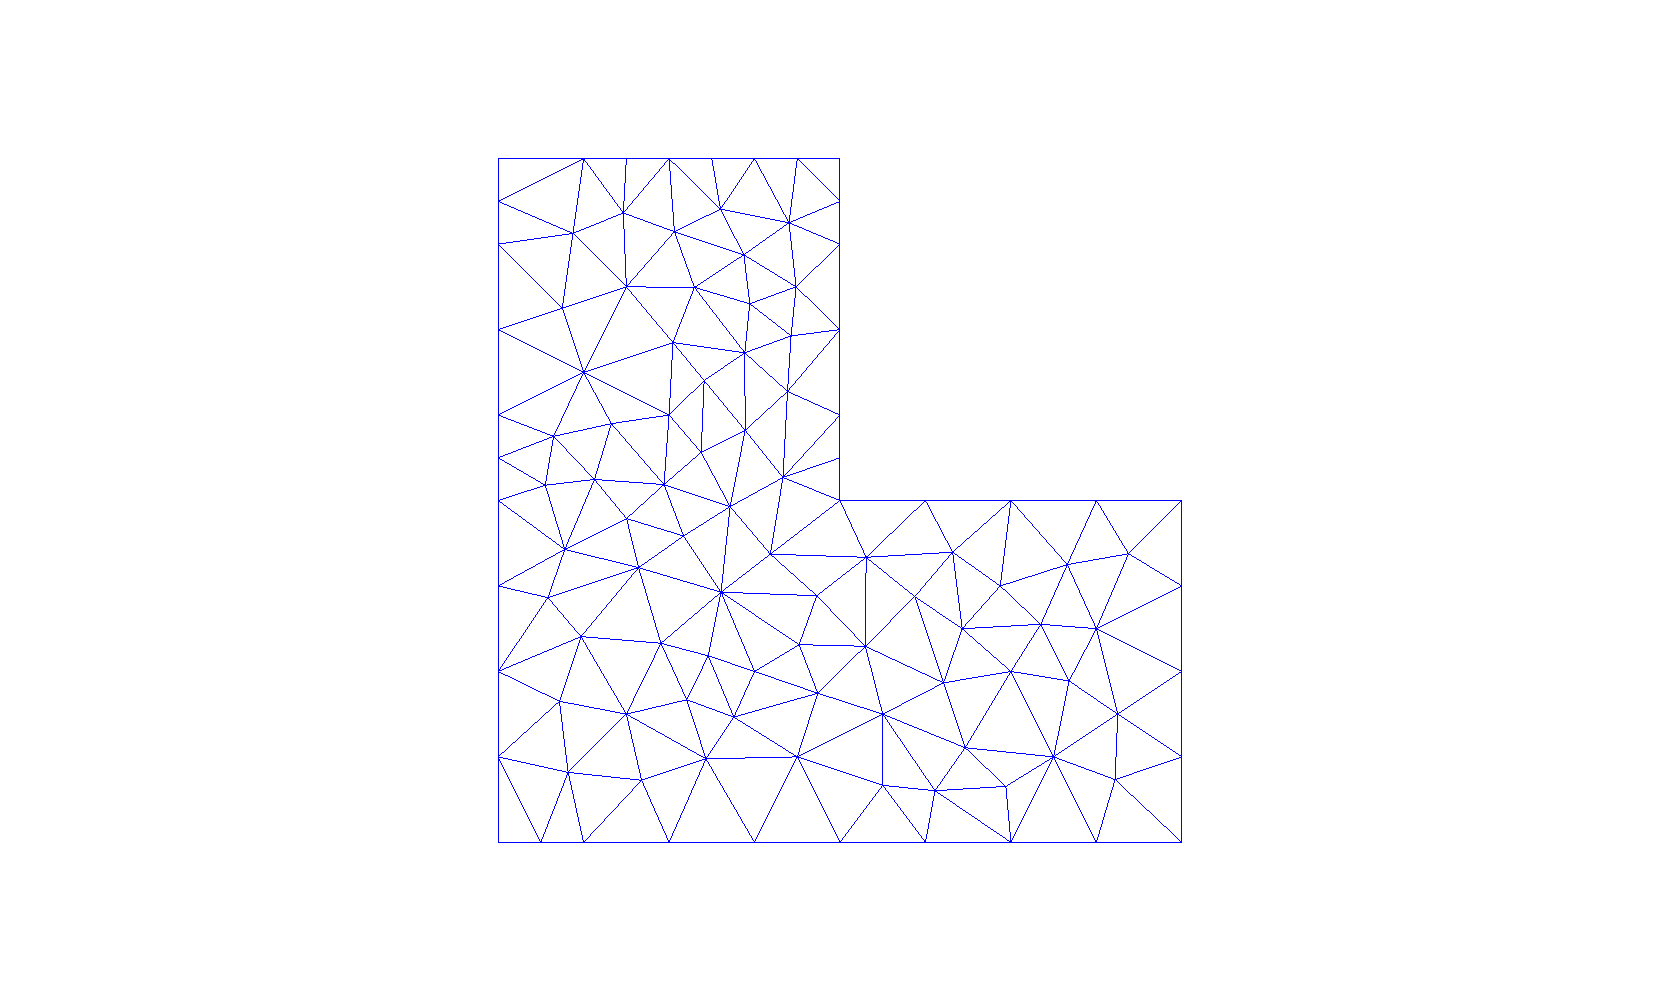
\includegraphics[width=0.6\textwidth]{../Lshaped.png}
    \caption{Lshaped domain}
    \label{fig:awesome_image}
\end{figure}
\section*{Preconditioner results - direct application of preconditioners}

\begin{table}[h!]
\centering
\begin{tabular}{ccccccccccc}
\hline
$\ell$ & DoF &  time$_{\rm solve}$ &  time$_{\rm NL}$ &  it$_{\rm NL}$ & it$_{\rm av}$ \\
\hline
1 &      71 & 0.00 & 0.29 & 15 & 22.0 \\
2 &     242 & 0.02 & 0.56 & 16 & 81.1 \\
3 &     909 & 0.03 & 1.34 & 24 & 59.8 \\
4 &    3,283 & 0.08 & 4.14 & 29 & 52.2 \\
5 &   12,867 & 0.35 & 16.91 & 30 & 52.1 \\
6 &   51,379 & 1.87 & 85.92 & 31 & 52.8 \\
7 &  203,556 & 12.37 & 504.08 & 31 & 53.8 \\
\hline
\end{tabular}
\end{table}

\newpage

\section*{Convergence results - direct solves on linear system}

\begin{table}[h!]
\begin{center}
\begin{tabular}{cccccccccc}
\hline
$\ell$ &    Dofs $\uu{u}_h/p_h$ & $\|\uu{u}-\uu{u}_h\|_{L^2(\Omega)}$ & order & $\|\uu{u}-\uu{u}_h\|_{H^1(\Omega)}$ & order  &  $\|{p}-{p}_h\|_{L^2(\Omega)}$ & order \\
\hline
 1 & 42/8 &  8.8613e+00 &     0.00 &  5.5371e+01 &     0.00 &  4.5613e+02 &      0.00 \\
 2 & 146/23 &  4.1281e+00 &     1.10 &  4.5019e+01 &     0.30 &  1.0459e+02 &      2.12 \\
 3 & 554/78 &  6.5366e-01 &     2.66 &  1.2378e+01 &     1.86 &  2.7443e+01 &      1.93 \\
 4 & 2,010/268 &  1.1755e-01 &     2.48 &  2.9325e+00 &     2.08 &  4.6939e+00 &      2.55 \\
 5 & 7,898/1,020 &  2.5188e-02 &     2.22 &  8.7477e-01 &     1.75 &  1.1816e+00 &      1.99 \\
 6 & 31,578/4,012 &  6.3267e-03 &     1.99 &  2.7412e-01 &     1.67 &  3.3121e-01 &      1.83 \\
 7 & 125,186/15,777 &  1.4864e-03 &     2.09 &  7.4636e-02 &     1.88 &  7.6414e-02 &      2.12 \\
\hline
\end{tabular}
\caption{Convergence of velocity/pressure field}
\label{tab:NS_2D_smooth_velocity}
\end{center}
\end{table}


\begin{table}[h!]
\begin{center}
\begin{tabular}{cccccc}
\hline
$\ell$ &    Dofs $\uu{b}_h/r_h$ & $\|\uu{b}-\uu{b}_h\|_{L^2(\Omega)}$ & order & $\|\uu{b}-\uu{b}_h\|_{H({\rm curl},\Omega)}$ & order \\
\hline
1 &     13/8 &  9.8687e+00 &     0.00 &  1.2202e+01 &        0.00 \\
2 &     50/23 &  4.6256e+00 &     1.09 &  8.8619e+00 &        0.46 \\
3 &    199/78 &  1.8629e+00 &     1.31 &  4.6257e+00 &        0.94 \\
4 &    737/268 &  8.7549e-01 &     1.09 &  2.1267e+00 &        1.12 \\
5 &   2,929/1,020 &  4.2624e-01 &     1.04 &  1.0126e+00 &        1.07 \\
6 &  11,777/4,012 &  2.1315e-01 &     1.00 &  5.4336e-01 &        0.90 \\
7 &  46,816/15,777 &  1.0649e-01 &     1.00 &  2.6991e-01 &        1.01 \\
\hline
\end{tabular}
\caption{Convergence for magnetic field}
\label{tab:2D_maxwell_magnetic}
\end{center}
\end{table}
\begin{table}[h!]
\begin{center}
\begin{tabular}{cccccc}
\hline
$\ell$ &    Dofs $\uu{b}_h/r_h$ & $\|{r}-{r}_h\|_{L^2(\Omega)}$ & order & $\|{r}-{r}_h\|_{H^1(\Omega)}$ & order\\
\hline
 1 &      13/8 &     9.7025e-01 &     0.00 &  1.0103e+01 &     0.00 \\
 2 &     50/23 &     1.5270e+00 &     0.65 &  1.2310e+01 &     0.29 \\
 3 &     199/78 &     4.3060e-01 &     1.83 &  5.0480e+00 &     1.29 \\
 4 &    737/268 &     8.5258e-02 &     2.34 &  2.3952e+00 &     1.08 \\
 5 &   2,929/1,020 &    2.2436e-02 &     1.93 &  1.1695e+00 &     1.03 \\
 6 &   11,777/4,012 &    5.4642e-03 &     2.04 &  5.7658e-01 &     1.02 \\
 7 &  46,816/15,777 &  1.3809e-03 &     1.98 &  2.9065e-01 &     0.99 \\

\hline
\end{tabular}
\caption{Convergence for  multiplier variable}
\label{tab:2D_maxwell_multiplier}

\end{center}
\end{table}



\end{document}

\chapter{Conclusion}

\bibliographystyle{plain}
\bibliography{../ref/ref}

\end{document}
\endinput
%%
%% End of file `ubcsample.tex'.
